\section{Problemas}

\begin{section-problem}
    Find the number of rational numbers $r$, $0 < r < 1$, such that when $r$ is written as a fraction in the lowest terms, the numerator and the denominator have a sum of 1000.
\end{section-problem}

\begin{section-problem}
    Each unit square of $4 \times 4$ square grid is colored either red, green or blue.
    Over all possible coloring of the grid, what is the maximun possible number of L-trominos that contain exactly one square of each color? (L-trominos are made up of three unit squares sharing a corner, as shown below.)
    \begin{figure}[htb]
        \centering
        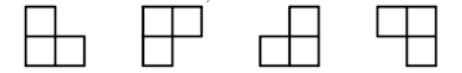
\includegraphics[width=8cm]{images/problem 2}
    \end{figure}
\end{section-problem}

\begin{section-problem}
    You see four statements.
    Select which of them are true.
    \begin{itemize}
        \item If the number $2^n - 1$ is prime for some positive integer $n$ then $n$ is prime.
        \item Call positive integer number $k$ \textit{good} if for any integer $a$ the number $a^k - a$ is divisible by 1001.
        The smallest good number greater than 1 is 721.
        \item Given prime number $p = 2017$.
        Numbers $0^{21}$, $1^{21}$, $2^{21}$, $\cdots$, $(p - 1)^{21}$ have distinct remainders modulo $p$.
        \item For any positive integer $k$ there are infinitely prime numbers $p$ such that $k$ is a square residue modulo $p$.
    \end{itemize}
\end{section-problem}

\begin{section-problem}
    Briefly tell what is wrong with this solution.

    \textbf{Problem.} The residential are has the shape of a rectangle divided by $a$ vertica and $b$ horizontal lines into $(a + 1)(b + 1)$ rectangular plots.
    The inspector can find out the area of any small rectangle.
    Whate is the smallest number of questions enough to findf out the area of the entire area?

    \textbf{Answer:} $a + b + 1$.

    \textbf{Solution.} We are going to prove the following statement: For an integer $n \geq 0$, the following is true: for any non-negative integers $a$ and $b$ whose sum is $n$, at least $n + 1$ question is needed.

    Base $n = 0$.
    We have only one small rectangle, we need to ask a question about its are.

    Step $n \to n + 1$.
    Let's take any $a$ and $b$ with the sum of $n + 1$.
    Since $n + 1 > 0$, then one of the numbers $a$ or $b$ is greater than zero.
    We can assume that $a > 0$.
    Consider the last column.
    Obviously, it is necessary to ask about at least one section from this column.
    Consider the remaining rectangle $(a) \times (b + 1)$.
    Acoording to the assumption of induction, it needs at least $(a - 1) + b + 1 = n$ questions.
    Another question is needed for the last column, so a total of $n + 1$ question is needed.
\end{section-problem}

\begin{section-problem}
    Bob was given a problem.
    \textit{Integer $a$ and $b$ satisfy $(\sqrt {3} + 2)^n = a + b\sqrt {3}$.
    Prove that $a^2 - 3b^2 = 1$.}
    Bob wrote the following solution.
    Denote $a_n$ and $b_n$ as integers satisfying $(\sqrt {3} + 2)^n = a_n + b_n \sqrt {3}$.
    We'll prove $a_n^2 - 3b_n^2 = 1$ using induction.
    Base case for $n = 1$ is obvious because $a_1 = 2, b_1 = 1$.
    For induction step you need to note that
    \[
        \left(\sqrt {3} + 2\right)^{n + 1} = \left(a_n + b_n \sqrt {3}\right)\left(2 + \sqrt {3}\right) = 2a_n + 3b_n + (a_n + 2b_n)\sqrt {3}.
    \]
    Hence $a_{n + 1} = 2a_n + 3b_n$ and $b_{n + 1} = a_n + 2b_n$.
    Let's prove that $\left(2a_n + 3b_n\right)^2 - 3\left(a_n + 2b_n\right)^2 = 1$.
    \[
        \left(2a_n + 3b_n\right)^2 - 3\left(a_n + 2b_n\right)^2 = (4 - 3)a_n^2 + (9 - 12)b_n^2 + (12 - 12)a_n b_n = a_n^2 - 4b_n^2 = 1.
    \]

    The teacher told that this solution is incomplete without lemma that $a_n$ and $b_n$ are always unique.
    Is the teacher correct?
    Try to explain your answer briefly.
\end{section-problem}

\begin{section-problem}
    An equiangular octagon $CAROLINE$, $CA = RO = LI = NE = \sqrt {2}$ and $AR = OL = IN = EC = 1$.
    The self-intersecting octagon $CORNELIA$ enclosed six non-overlapping triangular regions.
    Let $K$ be the area enclosed by $CORNELIA$, that is, the total area of the six triangular regions.
    Then $K = \frac{a}{b}$, where $a$ and $b$ are relatively prime positive integers.
    Find $a + b$.
    \begin{figure}[htb]
        \centering
        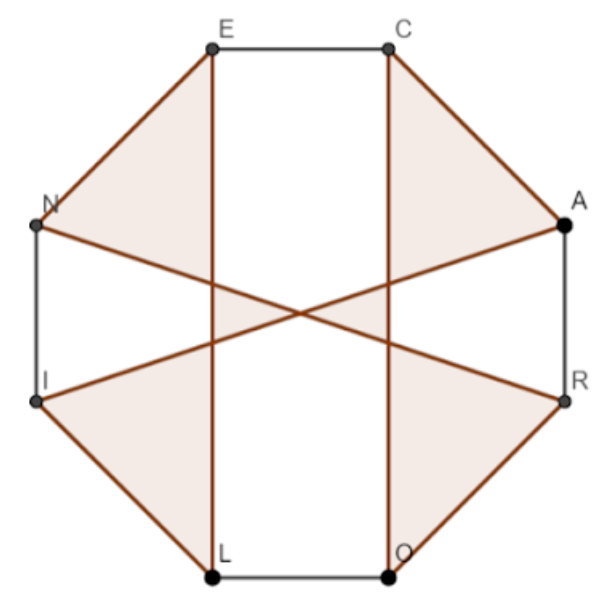
\includegraphics[width=6cm]{images/problem 6}
    \end{figure}
\end{section-problem}

\begin{section-problem}
    Let $x_1 < x_2 < x_3$ be the three real roots of the equation $\sqrt {2014} x^3 - 4029 x^2 + 2 = 0$.
    Find $x_2\left(x_1 + x_3\right)$.
\end{section-problem}